
% part 14

% When a Deferred Isn’t
\section{Случай, когда Deferred не является Deferred'ом\label{sec:part14}}

\subsection{Введение}


В этой части мы изучим другую сторону класса Deffered. 
Для мотивации нашего обсуждения, давайте добавим еще один сервер в наши 
стабильные поэтические сервисы. Предположим, что есть большое 
количество внутренних клиентов, которые хотят получить поэзию из 
одного и того же внешнего сервера. Но этот внешний сервер медленный 
и уже перегружен ненасытными сетевыми поэтическими запросами. Мы не 
хотим перегружать этот несчастный сервер, отправляя туда всех наших клиентов.  


Поэтому вместо этого мы сделаем кеширующий прокси сервер. Когда 
клиент подсоединяется к прокси, прокси либо вытащит поэму из 
внешнего сервера, либо вернет закешированную копию 
поэмы, полученную ранее. Затем мы можем указать клиентам на прокси, 
после чего нагрузка на сервер спадет. Эта система 
показана на рисунке \ref{fig:proxy1}:

% fig30
\begin{figure}[h]
\begin{center}
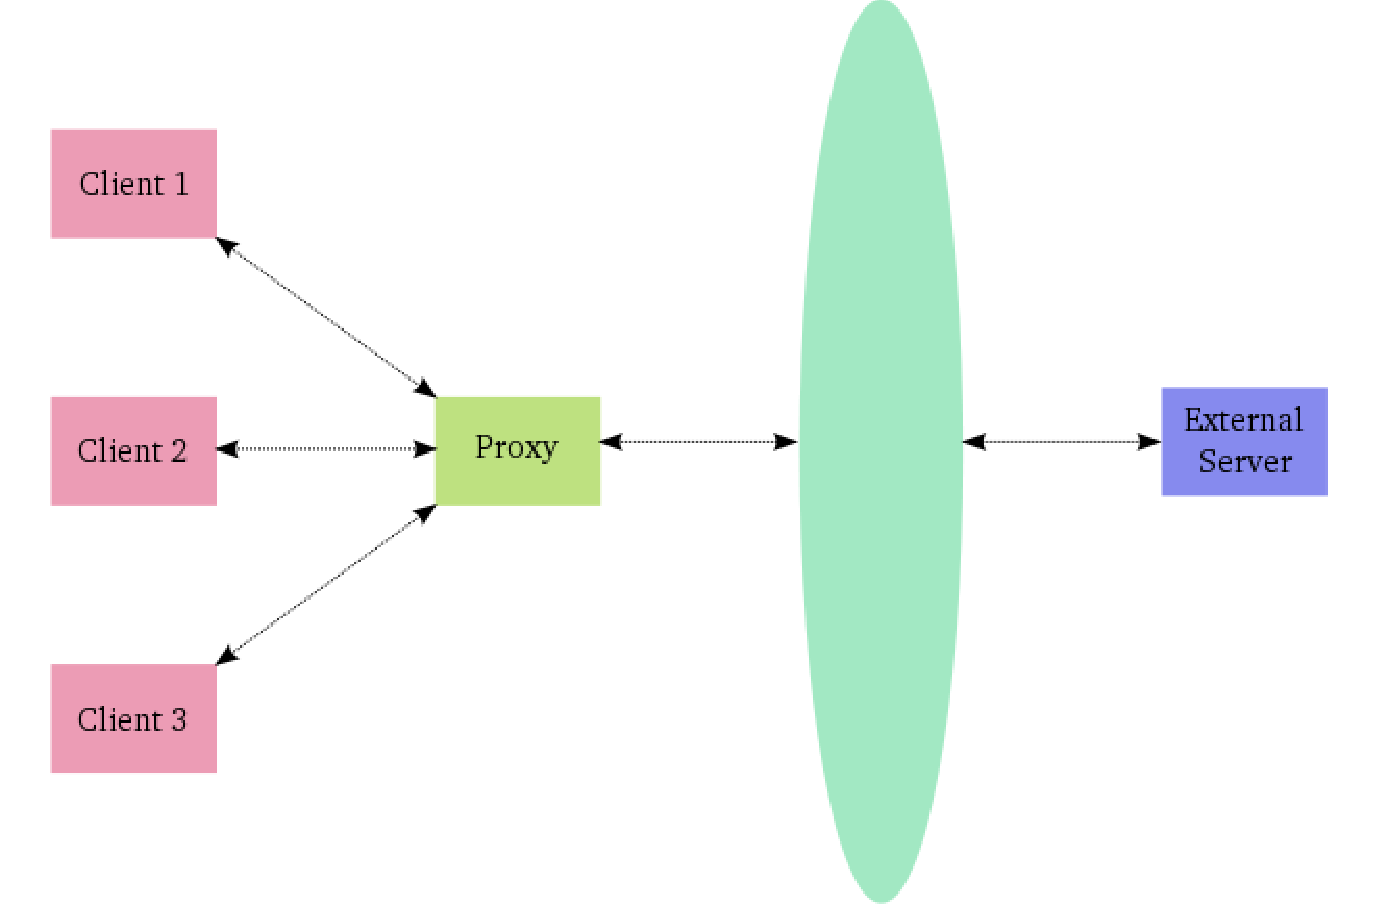
\includegraphics[width=0.8\textwidth]{images/proxy1.pdf} 
\caption{Кеширующий прокси сервер}\label{fig:proxy1}
\end{center}
\end{figure}

Рассмотрим что случится, когда клиент подсоединится к 
прокси для получения поэмы. Если кеш пустой, то прокси должен 
ждать (асинхронно) пока внешний сервер ответит до того, как 
отправить поэму. Пока все хорошо, и мы уже знаем как управлять 
такой ситуацией используя асинхронную функцию, которая 
возвращает deferred. С другой стороны, если в кеше уже есть поэма, 
то прокси может отправить ее обратно немедленно без ожидания. 
Поэтому внутренний механизм прокси для получения поэмы 
будет иногда асинхронным, а иногда - синхронным.


Что нам делать, если мы хотим иметь функцию, которая 
асинхронная только иногда? Twisted предоставляет ряд 
опций, зависящих от свойств класса Deferred, 
которые мы еще не использовали: вы можете активизировать 
deferred до того, как вы возвратите его тому, кто его вызывал. 


Это работает, поскольку вы не можете активизировать 
deferred дважды, вы можете добавить callback'и и 
errback'и в deferred после того, как он уже был активизирован. 
И когда вы так делаете, deferred просто продолжает 
активизировать цепочку с того места, на котором он остановился. 
Одна важная вещь, про которую надо упомянуть: один раз 
активизированный deferred может активизировать новый callback (или 
errback, взависимости от состояния deferred'а) сразу же, например, 
после его добавления. 

Рассмотрим рисунок \ref{fig:deferred-13}, показывающий deferred, 
который был активизирован:

% fig31
\begin{figure}[h]
\begin{center}
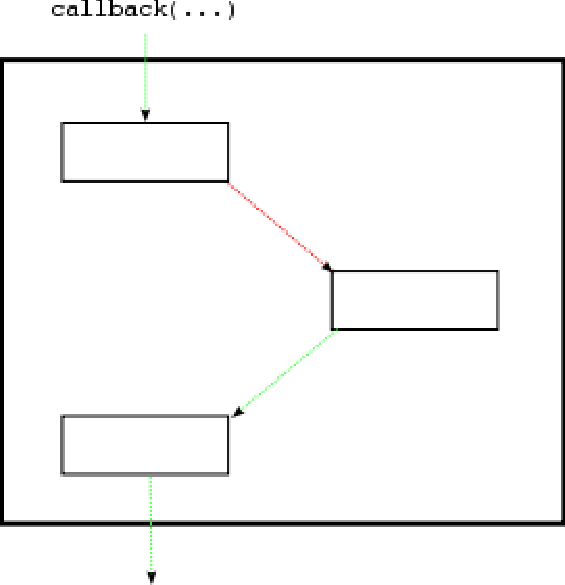
\includegraphics[height=0.3\textheight]{images/deferred-13.pdf} 
\caption{Активизированный deferred}\label{fig:deferred-13}
\end{center}
\end{figure}

Если бы мы добавили другую пару callback/errback 
в этом месте, то deferred сразу же активизировал новый 
callback, как это показано на рисунке \ref{fig:deferred-14}.

% fig32
\begin{figure}[h]
\begin{center}
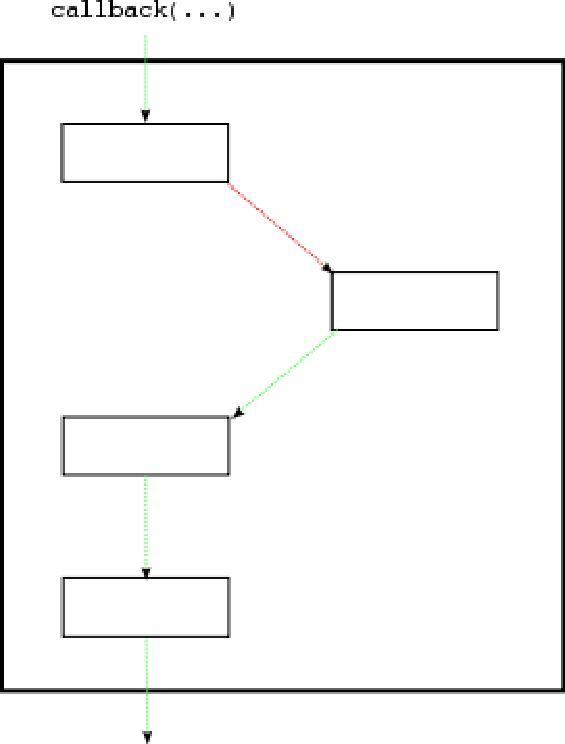
\includegraphics[height=0.3\textheight]{images/deferred-14.pdf} 
\caption{Тот же deferred с новым callback'м}\label{fig:deferred-14}
\end{center}
\end{figure}


Активизация callback (не errback) происходит, потому что 
предыдущий callback завершился без ошибок. Если бы он 
завершился с ошибкой (вызвал Exception или возвратил Failure), 
то был бы вызван новый errback.


Мы можем проверить описанные новые свойства, используя пример кода из 
\href{http://github.com/jdavisp3/twisted-intro/blob/master/twisted-deferred/defer-11.py#L1}{twisted-deferred/defer-11.py}. Прочитайте и запустите этот скрипт, 
для того, чтобы посмотреть как deferred ведут себя, когда 
вы их сначала активизируете и затем добавляете callback'и. 
Заметьте, что в первом примере каждый новый callback 
вызывается сразу же (вы можете сказать, что со скоростью порядка вывода 
с использованием print).


Второй пример в этом скрипте показывает, как вы можете 
приостановить, используя  
\href{http://twistedmatrix.com/trac/browser/tags/releases/twisted-8.2.0/twisted/internet/defer.py#L272}{pause()}, deferred так, чтобы он не активизировал 
callback'и прямо сейчас. Когда мы готовы для 
активизации callback'в, мы вызовем 
\href{http://twistedmatrix.com/trac/browser/tags/releases/twisted-8.2.0/twisted/internet/defer.py#L278}{unpause()}. Это в точности тот же механизм, который 
используют deferred'ы для приостановки 
самих себя, когда один из их callback'в возвращает другой deferred. 

\subsection{Прокси 1.0}

Теперь давайте посмотрим на первую версию 
поэтического прокси в 
\href{http://github.com/jdavisp3/twisted-intro/blob/master/twisted-server-1/poetry-proxy.py#L1}{twisted-server-1/poetry-proxy.py}. С того момента как 
прокси работает и как клиент, и как сервер, он имеет две 
пары Protocol/Factory классов, одна из них обслуживает 
поэзию, другая пара - получает поэзию из внешнего сервера. 
Мы не будем рассматривать код клиентской пары, она аналогична 
рассмотренной ранее.

Но до того как мы посмотрим на серверную пару, мы посмотрим 
на \href{http://github.com/jdavisp3/twisted-intro/blob/master/twisted-server-1/poetry-proxy.py#L100}{ProxyService}, который использует протокол на стороне 
сервера для получения поэмы:

\begin{scriptsize}\begin{verbatim}
class ProxyService(object):

    poem = None # the cached poem

    def __init__(self, host, port):
        self.host = host
        self.port = port

    def get_poem(self):
        if self.poem is not None:
            print 'Using cached poem.'
            return self.poem

        print 'Fetching poem from server.'
        factory = PoetryClientFactory()
        factory.deferred.addCallback(self.set_poem)
        from twisted.internet import reactor
        reactor.connectTCP(self.host, self.port, factory)
        return factory.deferred

    def set_poem(self, poem):
        self.poem = poem
        return poem
\end{verbatim}\end{scriptsize}


Здесь ключевой метод - get\_poem. Если в кеше уже есть поэма, 
то метод просто возвращает саму поэму. С другой стороны, 
если мы еще не получили поэму, мы инициируем соединение 
к внешнему серверу и возвращаем deferred, который будет активизирован, 
когда прийдет поэма. Поэтому get\_poem - функция, являющаяся 
иногда асинхронной.

Как управлять функцией, подобной этой? Давайте посмотрим на пару 
\href{http://github.com/jdavisp3/twisted-intro/blob/master/twisted-server-1/poetry-proxy.py#L52}{protocol/factory} на стороне сервера:

\begin{scriptsize}\begin{verbatim}
class PoetryProxyProtocol(Protocol):

    def connectionMade(self):
        d = maybeDeferred(self.factory.service.get_poem)
        d.addCallback(self.transport.write)
        d.addBoth(lambda r: self.transport.loseConnection())

class PoetryProxyFactory(ServerFactory):

    protocol = PoetryProxyProtocol

    def __init__(self, service):
        self.service = service
\end{verbatim}\end{scriptsize}


Класс PoetryProxyFactory простой: он просто сохраняет 
ссылку на прокси сервис, так что экземпляры PoetryProxyProtocol 
могут вызывать метод get\_poem. PoetryProxyFactory - место, где 
происходят все действия. Вместо вызова get\_poem напрямую, 
PoetryProxyFactory использует обертку из модуля twisted.internet.defer 
\href{http://twistedmatrix.com/trac/browser/tags/releases/twisted-8.2.0/twisted/internet/defer.py#L84}{maybeDeferred}.


Функция maybeDeferred берет ссылку на другую функцию, 
плюс некоторые опциональные аргументы для этой 
функции (мы их не используем). После этого maybeDeferred 
действительно вызовет эту функцию и:

\begin{itemize}

\item Если функция возвращает deferred, maybeDeferred 
возвращает тот же deferred

\item Если функция возвращает Failure, maybeDeferred 
возвращает новый deferred, который активизировался (через 
.errback()) c этим Failure

\item Если функция возвращает обычное значение, maybeDeferred 
возвращает deferred, который активизировался с этим значением в 
качестве аргумента result

\item Если функция сгенерировала исключение, maybeDeferred 
возвращает deferred, который активизировался (через .errback()) с 
этим исключением, обернутым в Failure.

\end{itemize}


Другими словами, возвращаемое значение функции maybeDeferred 
является гарантированно deferred'ом, даже если функция, которую 
вы подставляете, никогда не возвращает deferred. Это позволяет 
нам безопасно вызывать синхронные функции (даже те, выполнение 
которых завершается исключением) и обрабатывать их как 
асинхронные функции, возвращающие deffered.


Замечание 1: Хотя, тонкое отличие все же будет. deferred, возвращенный 
синронной функцией, уже активизирован, поэтому любые callback'и или 
errback'и, которые вы добавили, запустятся немедленно, а не в 
некотором будущем взаимодействии цикла реактора.


Замечание 2: По недосмотрительности, пожалуй, называть функцию, 
которая всегда возвращает deferred, ``maybeDeferred'' - было не 
лучшим выбором.


Поскольку PoetryProxyProtocol имеет реальный deferred для 
управления, он может добавить некоторые callback'и, 
которые отправляют поэму клиенту и затем закрывают 
соединение. 


\subsection{Запуск прокси}

Для того, чтобы попробовать прокси, запустите поэтический сервер:

\begin{scriptsize}\begin{verbatim}
python twisted-server-1/fastpoetry.py --port 10001 poetry/fascination.txt
 \end{verbatim}\end{scriptsize}

И теперь запустите прокси сервер:

то \begin{scriptsize}\begin{verbatim}
python twisted-server-1/poetry-proxy.py --port 10000 10001
\eто nd{verbatim}\end{scriptsize}


Это должно говорить вам, что проксирующая поэзия на 
порту 10000 для сервера на порту 10001. Теперь вы можете 
указать клиенту прокси:

\begin{scriptsize}\begin{verbatim}
python twisted-client-4/get-poetry.py 10000
\end{verbatim}\end{scriptsize}


Мы будем использовать предыдущую версию клиента, 
которая не связана с поэтическими преобразованиями. вы 
увидите поэму в клиентском окне и текст в окне с 
запущенным прокси, в котором будет 
запись о том, что прокси скачивает поэму с сервера. Теперь снова 
запустите клиент, и прокси должен подтвердить, что он использует 
закешированную версию поэмы, в то время как клиент показывает 
ту же поэму, что и раньше. 


\subsection{Прокси 2.0}


Как мы упомянули ранее, существует альтернативный способ 
реализовать такую схему. Это показано в поэтическом прокси 
версии 2.0, расположенном в 
\href{http://github.com/jdavisp3/twisted-intro/blob/master/twisted-server-2/poetry-proxy.py#L1}{twisted-server-2/poetry-proxy.py}. Поскольку мы можем 
активизировать deferred'ы до того, как мы их 
возвратим, мы можем создать прокси сервис, возвращающий 
уже активизированный deferred, в случае присутсвия поэмы в 
кеше. Далее новая версия метода get\_poem в прокси сервисе:

\begin{scriptsize}\begin{verbatim}
    def get_poem(self):
        if self.poem is not None:
            print 'Using cached poem.'
            # return an already-fired deferred
            return succeed(self.poem)

        print 'Fetching poem from server.'
        factory = PoetryClientFactory()
        factory.deferred.addCallback(self.set_poem)
        from twisted.internet import reactor
        reactor.connectTCP(self.host, self.port, factory)
        return factory.deferred
\end{verbatim}\end{scriptsize}


Функция \href{http://twistedmatrix.com/trac/browser/tags/releases/twisted-8.2.0/twisted/internet/defer.py#L30}{defer.succeed} - это просто удобный способ создать уже 
активизированный deferred передавая ему результат. 
Просмотрите реализацию этой функции, и вы увидите, что 
это просто, по сути, создание нового deferred'а и его 
активизация с использованием .callback(). Если бы вы хотели 
возвратить активизированный deferred с ошибкой, вы могли бы 
использовать defer.fail.


В этой версии, поскольку get\_poem всегда возвращает 
deferred, класс PoetryProxyProtocol не нуждается больше 
в использование метода maybeDeferred (хотя, из изученного ранее, 
ясно, что он бы работал, если бы мы его оставили): 

\begin{scriptsize}\begin{verbatim}
class PoetryProxyProtocol(Protocol):

    def connectionMade(self):
        d = self.factory.service.get_poem()
        d.addCallback(self.transport.write)
        d.addBoth(lambda r: self.transport.loseConnection())

\end{verbatim}\end{scriptsize}


Кроме этих двух изменений вторая версия прокси аналогична первой, 
и вы можете запустить ее тем же образом, что и первоначальную.


\subsection{Резюме}

%In this Part we learned how deferreds can be fired before they are returned, and thus we can use them in synchronous (or sometimes synchronous) code. And we have two ways to do that:

В этой главе мы изучили как deferred'ы могут быть активизированы 
до того, как они были возвращены, и таким образом мы можем 
использовать их в синхронном (или частично синхронном) коде. 
И мы имеет два способа сделать это: 

\begin{itemize}

\item Мы можем использовать maybeDeferred для управления 
функцией, которая иногда возвращает deferred, а иногда - 
обычное значение (или бросает исключение);

\item Мы можем предактивизировать свои собственные 
deferred'ы, используя defer.succeed или defer.fail, 
поэтому наша ``полусинхронная'' функция всегда возвращает 
deferred.

\end{itemize}

Какую технику вы выбирете - дело ваше.
Первый вариант подчеркивает, что 
наша функция не всегда асинхронная, в то время 
как второй вариант упрощает клиентский код. 
Пожалуй, не существует однозначного аргумента 
при выборе одного вместо другого. 


Оба приема нужны для того, 
чтобы мы могли добавлять callback'и и errback'и к 
deferred'м, после того как они были активизированы. И 
это объясняет любопытный факт, который мы обнаружили 
в главе 9, и примере \href{http://github.com/jdavisp3/twisted-intro/blob/master/twisted-deferred/defer-unhandled.py#L1}{twisted-deferred/defer-unhandled.py}. Мы изучили, что 
``неуправляемая ошибка'' в deferred'е возникает в случае, когда последний  
callback или последний errback завершился с ошибкой, и это не сообщается 
до тех пор, пока deferred не будет утилизирован сборщиком мусора (например, 
когда в коде нет на него ссылок). 
Теперь мы знаем почему: поскольку мы могли всегда 
добавить еще одну callback/errback пару в deferred, 
которая управляет той ошибкой, и не активизируется, 
чтобы Twisted мог сказать, что ошибка не обработана, 
до тех пор, пока есть ссылки.


Теперь, когда вы потратили так много времени, исследуя 
класс Deferred, который расположен в пакете twisted.internet, 
вы могли бы заметить, что он ничего не должен делать с Internet. 
Это просто абстракция для управления callback'ми. Так что же он там 
делает? Это артифакт истории Twisted. В лучшем из всех 
возможных миров, модуль для deferred'в вероятнее был бы в twisted.python. 
Полагаю, что такова жизнь.  


Так что это за deferred'ы? Знаем ли мы все о их свойствах? 
По большей части - да. Но Twisted позволяет использовать 
альтернативные способы использования deferred'в, которые 
мы еще не исследовали (мы доберемся!). Тем временем, 
разработчики Twisted упорно работают над добавлением новой 
вещи. В новом релизе, класс Deferred преобретен новую 
возможность. Мы ознакомимся с ней в следующей главе, но 
сначала, мы прервем изучение deferred'в и посмотрим 
на некоторые стороны Twisted, включая тестирование.


\subsection{Упражнения}


\begin{enumerate}

\item Модифицируйте пример 
\href{http://github.com/jdavisp3/twisted-intro/blob/master/twisted-deferred/defer-11.py#L1}{twisted-deferred/defer-11.py} для иллюстрации предактивизированный ошибкой deferred'в, 
используя .errback(). Прочтите докуменатцию и реализацию функции defer.fail.

\item Модифицируйте прокси так, чтобы закешированная более 2 часов поэма отбрасывалась, 
вызывая перезапрос из сервера следующего запроса.

\item Предполагается, что прокси избегает присоединения к серверу более 
одного раза, но при нескольких клиентских запросах, приходящих 
одновременно во время отсутвия поэмы в кеше, прокси будет делать 
несколько поэтических запросов. Это проще увидеть, если вы используете 
медленный сервер для проверки. 

Поменяйте прокси-сервис так, 
чтобы генерировался только один запрос. Сейчас 
сервис имеет только два состояния: либо поэма к кеше, либо - не в кеше. 
вам нужно добавить третье состояние, показывающее, что запрос был сделан, 
но еще не завершен. Когда метод get\_poem вызывается в третьем состоянии, 
добавьте новый deferred в список ``ожидающих''. Этот новый deferred 
будет результатом от метода get\_poem. Когда поэма окончательно 
вернется, активизируйте все ожидающие deferred'ы с поэмой и 
перейдите в закешированной состояние. Если в процессе ожидания поэмы 
возникла ошибка, то активизируйте метод .errback() для 
всех ожидающих deferred'ов и перейдите в незакешированное состояние.  

\item Добавьте преобразующий прокси в прокси-сервис. Этот сервис должен 
работать так же, как изначальный преоразующий сервис, но использовать 
внешний сервер для того, чтобы осуществить трансформации. 

\item Предположим следующий гипотетический кусок кода:

\begin{scriptsize}\begin{verbatim}
      d = some_async_function() # d is a Deferred
      d.addCallback(my_callback)
      d.addCallback(my_other_callback)
      d.addErrback(my_errback)
\end{verbatim}\end{scriptsize}

Предположим, что когда deferred d возвращен в строке 1, 
он не активизирован. Возможно ли для этого deferred'а, что 
он будет активизирован в момент, когда мы добавляем наши 
callback'и и errback'и в строках 2-4? Почему да или почему нет?

\end{enumerate}

